
% THIS IS AN EXAMPLE DOCUMENT FOR VLDB 2012
% based on ACM SIGPROC-SP.TEX VERSION 2.7
% Modified by  Gerald Weber <gerald@cs.auckland.ac.nz>
% Removed the requirement to include *bbl file in here. (AhmetSacan, Sep2012)
% Fixed the equation on page 3 to prevent line overflow. (AhmetSacan, Sep2012)

\documentclass{vldb}
\usepackage{graphicx}
\usepackage{balance}  % for  \balance command ON LAST PAGE  (only there!)

% ****************** sungsoo's packages ****************************************
\usepackage{times}
%                              My Commands
\newcommand{\bi}{\begin{itemize}}
\newcommand{\ei}{\end{itemize}}
\newcommand{\be}{\begin{enumerate}}
\newcommand{\ee}{\end{enumerate}}
\newcommand{\ii}{\item}
\newtheorem{Def}{Definition}
\newtheorem{Lem}{Lemma}
\usepackage{algorithm}
\usepackage{algorithmicx}
\usepackage{algpseudocode}

\usepackage{graphicx}
\graphicspath{%
        {converted_graphics/}
        {./images/}
}
\usepackage{hyperref}
\usepackage{listings}
\usepackage{longtable}

% ****************** the following is needed for syntax highlighting
\usepackage{color}

\definecolor{dkgreen}{rgb}{0,0.6,0}
\definecolor{gray}{rgb}{0.5,0.5,0.5}
\definecolor{mauve}{rgb}{0.58,0,0.82}

\lstset{ %
  language=Java,                  % the language of the code
  basicstyle=\scriptsize,       % the size of the fonts that are used for the code
  numbers=left,                   % where to put the line-numbers
  numberstyle=\tiny\color{gray},  % the style that is used for the line-numbers
  stepnumber=1,                   % the step between two line-numbers. If it's 1, each line 
                                  % will be numbered
  numbersep=3.8pt,                  % how far the line-numbers are from the code
  backgroundcolor=\color{white},  % choose the background color. You must add \usepackage{color}
  showspaces=false,               % show spaces adding particular underscores
  showstringspaces=false,         % underline spaces within strings
  showtabs=false,                 % show tabs within strings adding particular underscores
  frame=false,                   % adds a frame around the code
  rulecolor=\color{black},        % if not set, the frame-color may be changed on line-breaks within not-black text (e.g. commens (green here))
  tabsize=2,                      % sets default tabsize to 2 spaces
  captionpos=b,                   % sets the caption-position to bottom
  breaklines=true,                % sets automatic line breaking
  breakatwhitespace=false,        % sets if automatic breaks should only happen at whitespace
  title=\lstname,                 % show the filename of files included with \lstinputlisting;
                                  % also try caption instead of title
  keywordstyle=\color{blue},          % keyword style
  commentstyle=\color{dkgreen},       % comment style
  stringstyle=\color{mauve},         % string literal style
  escapeinside={\%*}{*)},            % if you want to add a comment within your code
  morekeywords={*,...}               % if you want to add more keywords to the set
}
% ****************** end of sungsoo's packages ****************************************


\begin{document}

% ****************** TITLE ****************************************

%\title{A Sample {\ttlit Proceedings of the VLDB Endowment} Paper in LaTeX
%Format\titlenote{for use with vldb.cls}}

\title{Parallel Data Placement}

% possible, but not really needed or used for PVLDB:
%\subtitle{[Extended Abstract]
%\titlenote{A full version of this paper is available as\textit{Author's Guide to Preparing ACM SIG Proceedings Using \LaTeX$2_\epsilon$\ and BibTeX} at \texttt{www.acm.org/eaddress.htm}}}

% ****************** AUTHORS **************************************

% You need the command \numberofauthors to handle the 'placement
% and alignment' of the authors beneath the title.
%
% For aesthetic reasons, we recommend 'three authors at a time'
% i.e. three 'name/affiliation blocks' be placed beneath the title.
%
% NOTE: You are NOT restricted in how many 'rows' of
% "name/affiliations" may appear. We just ask that you restrict
% the number of 'columns' to three.
%
% Because of the available 'opening page real-estate'
% we ask you to refrain from putting more than six authors
% (two rows with three columns) beneath the article title.
% More than six makes the first-page appear very cluttered indeed.
%
% Use the \alignauthor commands to handle the names
% and affiliations for an 'aesthetic maximum' of six authors.
% Add names, affiliations, addresses for
% the seventh etc. author(s) as the argument for the
% \additionalauthors command.
% These 'additional authors' will be output/set for you
% without further effort on your part as the last section in
% the body of your article BEFORE References or any Appendices.

\numberofauthors{1} %  in this sample file, there are a *total*
% of EIGHT authors. SIX appear on the 'first-page' (for formatting
% reasons) and the remaining two appear in the \additionalauthors section.

\author{
% You can go ahead and credit any number of authors here,
% e.g. one 'row of three' or two rows (consisting of one row of three
% and a second row of one, two or three).
%
% The command \alignauthor (no curly braces needed) should
% precede each author name, affiliation/snail-mail address and
% e-mail address. Additionally, tag each line of
% affiliation/address with \affaddr, and tag the
% e-mail address with \email.
%
% 1st. author
\alignauthor
Sung-Soo Kim\\ %\titlenote{Dr.~Trovato insisted his name be first.}\\
       \affaddr{Data Management Research Section}\\
       \affaddr{Electronics and Telecommunications Research Institute}\\
       \affaddr{128 Gajeong-ro, Yuseong-gu}\\
       \affaddr{Daejeon, South Korea}\\
       \email{\normalsize \it sungsoo@etri.re.kr}
% 2nd. author
%\alignauthor
%G.K.M. Tobin\titlenote{The secretary disavows
%any knowledge of this author's actions.}\\
%       \affaddr{Institute for Clarity in Documentation}\\
%       \affaddr{P.O. Box 1212}\\
%       \affaddr{Dublin, Ohio 43017-6221}\\
%       \email{webmaster@marysville-ohio.com}
% 3rd. author
%\alignauthor Lars Th{\Large{\sf{\o}}}rv{$\ddot{\mbox{a}}$}ld\titlenote{This author is the
%one who did all the really hard work.}\\
%       \affaddr{The Th{\large{\sf{\o}}}rv{$\ddot{\mbox{a}}$}ld Group}\\
%       \affaddr{1 Th{\large{\sf{\o}}}rv{$\ddot{\mbox{a}}$}ld Circle}\\
%       \affaddr{Hekla, Iceland}\\
%       \email{larst@affiliation.org}
%\and  % use '\and' if you need 'another row' of author names
% 4th. author
%\alignauthor Lawrence P. Leipuner\\
%       \affaddr{Brookhaven Laboratories}\\
%       \affaddr{Brookhaven National Lab}\\
%       \affaddr{P.O. Box 5000}\\
%       \email{lleipuner@researchlabs.org}
% 5th. author
%\alignauthor Sean Fogarty\\
%       \affaddr{NASA Ames Research Center}\\
%       \affaddr{Moffett Field}\\
%       \affaddr{California 94035}\\
%       \email{fogartys@amesres.org}
% 6th. author
%\alignauthor Charles Palmer\\
%       \affaddr{Palmer Research Laboratories}\\
%       \affaddr{8600 Datapoint Drive}\\
%       \affaddr{San Antonio, Texas 78229}\\
%       \email{cpalmer@prl.com}
}
% There's nothing stopping you putting the seventh, eighth, etc.
% author on the opening page (as the 'third row') but we ask,
% for aesthetic reasons that you place these 'additional authors'
% in the \additional authors block, viz.
%\additionalauthors{Additional authors: John Smith (The Th{\o}rv\"{a}ld Group, {\texttt{jsmith@affiliation.org}}), Julius P.~Kumquat
%(The \raggedright{Kumquat} Consortium, {\small \texttt{jpkumquat@consortium.net}}), and Ahmet Sacan (Drexel University, {\small \texttt{ahmetdevel@gmail.com}})}
%\date{30 July 1999}
% Just remember to make sure that the TOTAL number of authors
% is the number that will appear on the first page PLUS the
% number that will appear in the \additionalauthors section.


\maketitle

\begin{abstract}
In this technical report, we describe the techniques for data placement in the parallel database systems. Many data-intensive applications require support for very large databases (e.g., hundreds of terabytes or petabytes).
Examples of such applications are e-commerce, data warehousing, and data mining. Very large databases are typically accessed through high numbers of concurrent transactions (e.g., performing on-line orders on an electronic store) or complex queries (e.g., decision-support queries). The first kind of access is representative of On-Line Transaction Processing (OLTP) applications while the second is representative of On-Line Analytical Processing (OLAP) applications. Supporting very large databases efficiently for either OLTP or OLAP can be addressed by combining parallel computing and distributed database management.

We describe five data partitioning schemes in the parallel database systems such as, \textit{round-robin}, \textit{hash}, \textit{range}, \textit{interleaved} and \textit{chained partitioning} schemes.
\end{abstract}


\section{Introduction}
In this technical report, we assume a \textit{shared-nothing architecture} because it is the most general case and its implementation techniques also apply, sometimes in a simplified form, to other architectures. Data placement in a parallel database system exhibits similarities with data fragmentation in distributed databases \cite{zsu:2011}. An obvious similarity is that fragmentation can be used to increase parallelism. 
In what follows, we use the terms \textit{partitioning} and \textit{partition} instead of horizontal fragmentation and horizontal fragment, respectively, to contrast with the alternative strategy, which consists of \textit{clustering} a relation at a single node. 
The term \textit{declustering} is sometimes used to mean partitioning. 
Vertical fragmentation can also be used to increase parallelism and load balancing much as in distributed databases. Another similarity is that since data are much larger than programs, execution should occur, as much as possible, where the data reside. 

However, there are two important differences with the distributed database approach. First, there is no need to maximize local processing (at each node) since users are not associated with particular nodes. Second, load balancing is much more difficult to achieve in the presence of a large number of nodes. The main problem is to avoid resource contention, which may result in the entire system thrashing (e.g., one node ends up doing all the work while the others remain idle). Since programs are executed where the data reside, data placement is a critical performance issue.

\section{Data Partitioning Strategies}

Data placement must be done so as to maximize system performance, which can be measured by combining the total amount of work done by the system and the response time of individual queries. We have seen that maximizing response time (through intra-query parallelism) results in increased total work due to communication overhead. For the same reason, inter-query parallelism results in increased total work. On the other hand, clustering all the data necessary to a program minimizes communication and thus the total work done by the system in executing that program. In terms of data placement, we have the following trade-off: maximizing response time or inter-query parallelism leads to partitioning, whereas minimizing the total amount of work leads to clustering. This problem is addressed in distributed databases in a rather static manner. The database administrator is in charge of periodically examining fragment access frequencies, and when necessary, moving and reorganizing fragments.

An alternative solution to data placement is \textit{full partitioning}, whereby each relation is horizontally fragmented across \textit{all} the nodes in the system. There are three basic strategies for data partitioning: \textit{round-robin}, \textit{hash}, and \textit{range partitioning} (Figure \ref{fig:partitioning}).

\begin{figure}[htb]
\centering
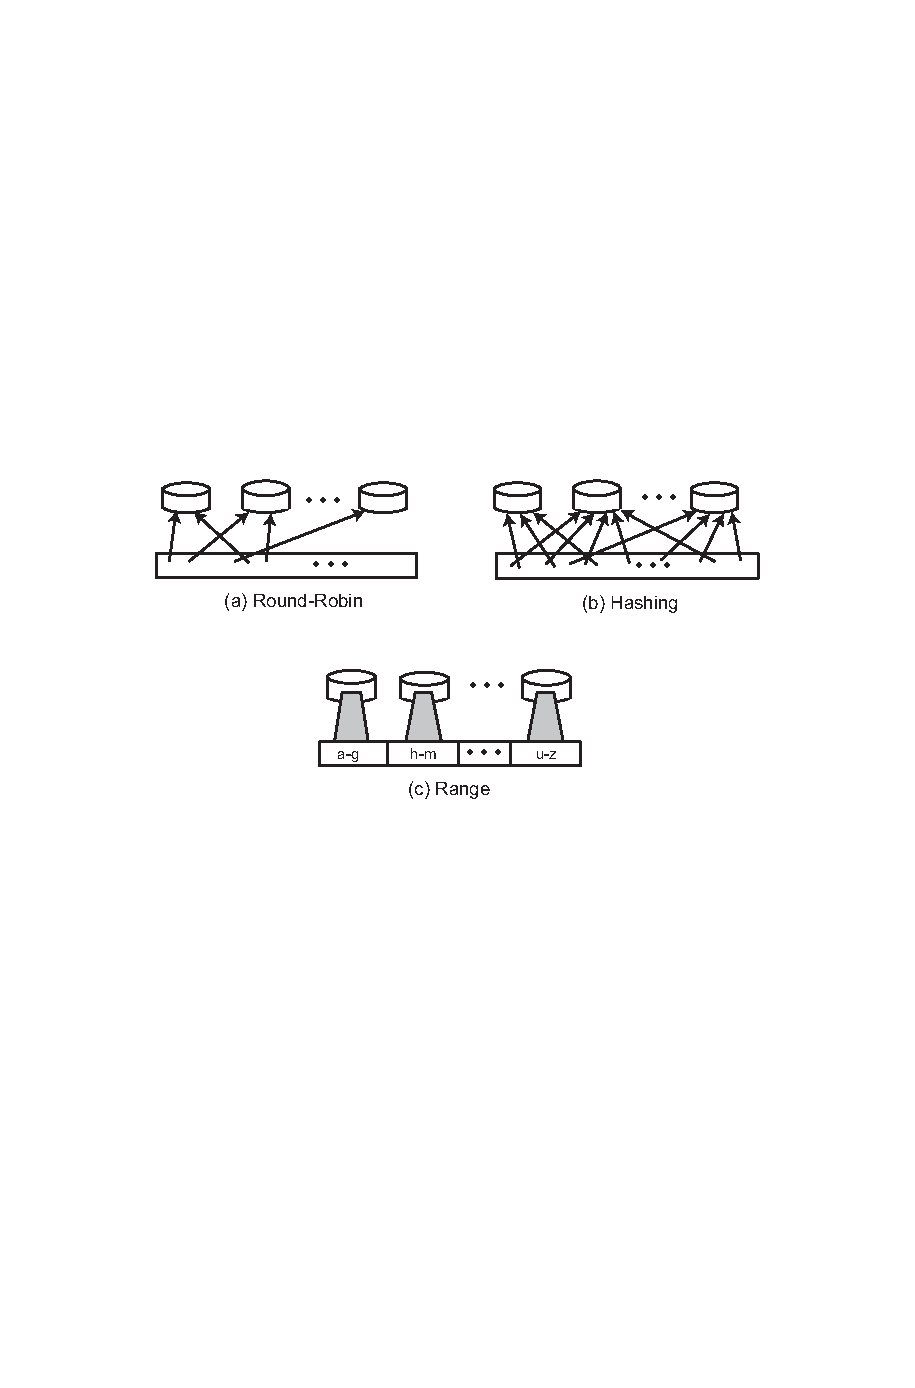
\includegraphics[width=0.48\textwidth]{partitioning}
\caption{Different Partitioning Schemes.}
\label{fig:partitioning}
\end{figure}
\be
\ii \textit{Round-robin partitioning} is the simplest strategy, it ensures uniform data distribution. 
With $n$ partitions, the $i$-th tuple in insertion order is assigned to partition ($i$ mod $n$). 
This strategy enables the sequential access to a relation to be done in parallel. However, the direct access to individual tuples, based on a predicate, requires accessing the entire relation.
\ii \textit{Hash partitioning} applies a hash function to some attribute that yields the partition number. This strategy allows exact-match queries on the selection attribute to be processed by exactly one node and all other queries to be processed by all the nodes in parallel.
\ii \textit{Range partitioning} distributes tuples based on the value intervals (ranges) of some attribute. In addition to supporting exact-match queries (as in hashing), it is well-suited for range queries. For instance, a query with a predicate “$A$ between $A_1$ and $A_2$” may be processed by the only node(s) containing tuples whose $A$ value is in range [$A_1$,$A_2$]. However, range partitioning can result in high variation in partition size.
\ee

Compared to clustering relations on a single (possibly very large) disk, full partitioning yields better performance. Although full partitioning has obvious performance advantages, highly parallel execution might cause a serious performance overhead for complex queries involving joins. Furthermore, full partitioning is not appropriate for small relations that span a few disk blocks. These drawbacks suggest that a compromise between clustering and full partitioning (i.e., \textit{variable partitioning}), needs to be found.

A solution is to do data placement by variable partitioning. The \textit{degree} of partitioning, i.e., the number of nodes over which a relation is fragmented, is a function of the size and access frequency of the relation. This strategy is much more involved than either clustering or full partitioning because changes in data distribution may result in reorganization. For example, a relation initially placed across eight nodes may have its cardinality doubled by subsequent insertions, in which case it should be placed across 16 nodes.

In a highly parallel system with variable partitioning, periodic reorganizations for load balancing are essential and should be frequent unless the workload is fairly static and experiences only a few updates. Such reorganizations should remain transparent to compiled programs that run on the database server. In particular, programs should not be recompiled because of reorganization. Therefore, the compiled programs should remain independent of data location, which may change rapidly. Such independence can be achieved if the run-time system supports associative access to distributed data. This is different from a distributed DBMS, where associative access is achieved at compile time by the query processor using the data directory.

\section{Data Placement}
\subsection{Global and Local Indexes}
One solution to associative access is to have a global index mechanism replicated on each node. The global index indicates the placement of a relation onto a set of nodes. Conceptually, the global index is a \textit{two-level index} with a major clustering on the relation name and a minor clustering on some attribute of the relation. This global index supports variable partitioning, where each relation has a different degree of partitioning. The index structure can be based on hashing or on a B-tree like organization. In both cases, exact match queries can be processed efficiently with a single node access. However, with hashing, range queries are processed by accessing all the nodes that contain data from the $r$ queried elation. Using a B-tree index (usually much larger than a hashed index) enables more efficient processing of \textit{range queries}, where only the nodes containing data in the specified range are accessed.

Figure \ref{fig:indexes} provides an example of a global index and a local index for relation EMP(ENO, ENAME, DEPT, TITLE) of the engineering database example.

\begin{figure}[htb]
\centering
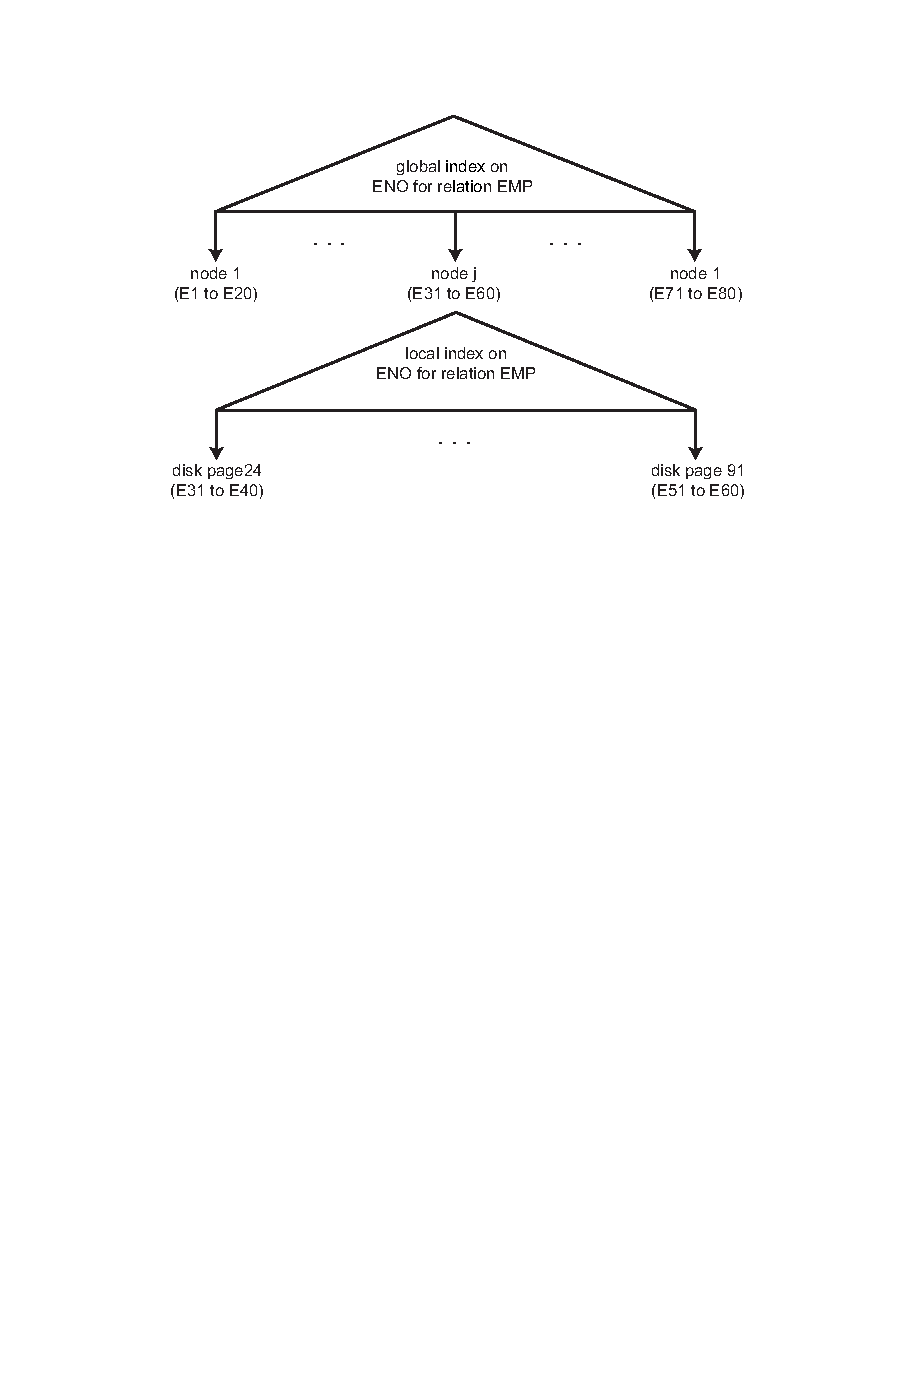
\includegraphics[width=0.48\textwidth]{indexes}
\caption{Example of Global and Local Indexes.}
\label{fig:indexes}
\end{figure}

Suppose that we want to locate the elements in relation EMP with ENO value “E50”. The first-level index on set name maps the name EMP onto the index on attribute ENO for relation EMP. Then the second-level index further maps the cluster value “E50” onto node number $j$. A local index within each node is also necessary to map a relation onto a set of disk pages within the node. The local index has two levels, with a major clustering on relation name and a minor clustering on some attribute. The minor clustering attribute for the local index is the same as that for the global index. Thus \textit{associative routing} is improved from one node to another based on (relation name, cluster value). This local index further maps the cluster value “E5” onto page number 91.

Experimental results for variable partitioning of a workload consisting of a mix of short transactions (debit-credit like) and complex ones indicate that as partitioning is increased, throughput continues to increase for short transactions. However, for complex transactions involving several large joins, further partitioning reduces throughput because of \textit{communication overhead}.

A serious problem in data placement is dealing with \textit{skewed data distributions} that may lead to non-uniform partitioning and hurt load balancing. Range partitioning is more sensitive to skew than either round-robin or hash partitioning. A solution is to treat non-uniform partitions appropriately, e.g., by further fragmenting large partitions. The separation between \textit{logical} and \textit{physical} nodes is also useful since a logical node may correspond to several physical nodes.

\subsection{Interleaved Partitioning}
A final complicating factor is \textit{data replication} for high availability. The simple solution is to maintain two copies of the same data, a primary and a backup copy, on two separate nodes. This is the \textit{mirrored disks} architecture promoted by many computer manufacturers. However, in case of a node failure, the load of the node with the copy may double, thereby hurting load balancing. To avoid this problem, several high-availability data replication strategies have been proposed for parallel database systems. An interesting solution is Teradata's interleaved partitioning that further partitions the backup copy on a number of nodes. Figure \ref{fig:interleaved} illustrates the interleaved partitioning of relation $R$ over four nodes, where each primary copy of a partition, e.g., $R_1$, is further divided in three partitions, e.g., $r_{11}$, $r_{12}$, and $r_{13}$, each at a different backup node. 
In failure mode, the load of the primary copy gets balanced among the backup copy nodes. But if two nodes fail, then the relation cannot be accessed thereby hurting availability. Reconstructing the primary copy from its separate backup copies may be costly. In normal mode, maintaining copy consistency may also be costly.
\begin{figure}[htb]
\centering
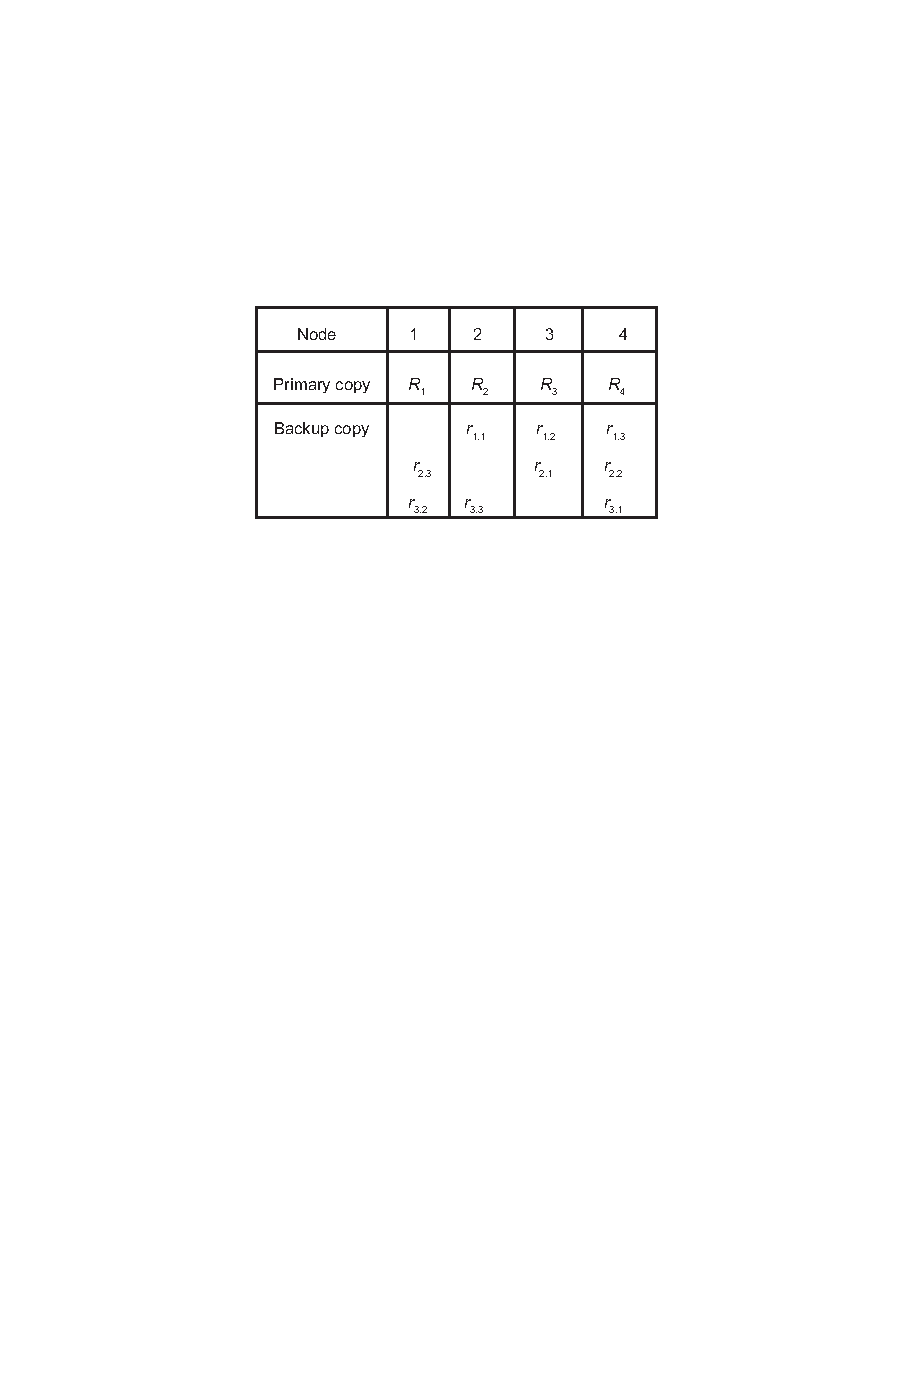
\includegraphics[width=0.48\textwidth]{interleaved}
\caption{Example of Interleaved Partitioning.}
\label{fig:interleaved}
\end{figure}

%\balance

\subsection{Chained Partitioning}
A better solution is Gamma’s \textit{chained partitioning}, which stores the primary and backup copy on two adjacent nodes (Figure \ref{fig:chained}). The main idea is that the probability that two adjacent nodes fail is much lower than the probability that any two nodes fail. In failure mode, the load of the failed node and the backup nodes are balanced among all remaining nodes by using both primary and backup copy nodes. In addition, maintaining copy consistency is cheaper. An open issue is how to perform data placement taking into account data replication. Similar to the fragment allocation in distributed databases, this should be considered an \textit{optimization problem}.

\begin{figure}[htb]
\centering
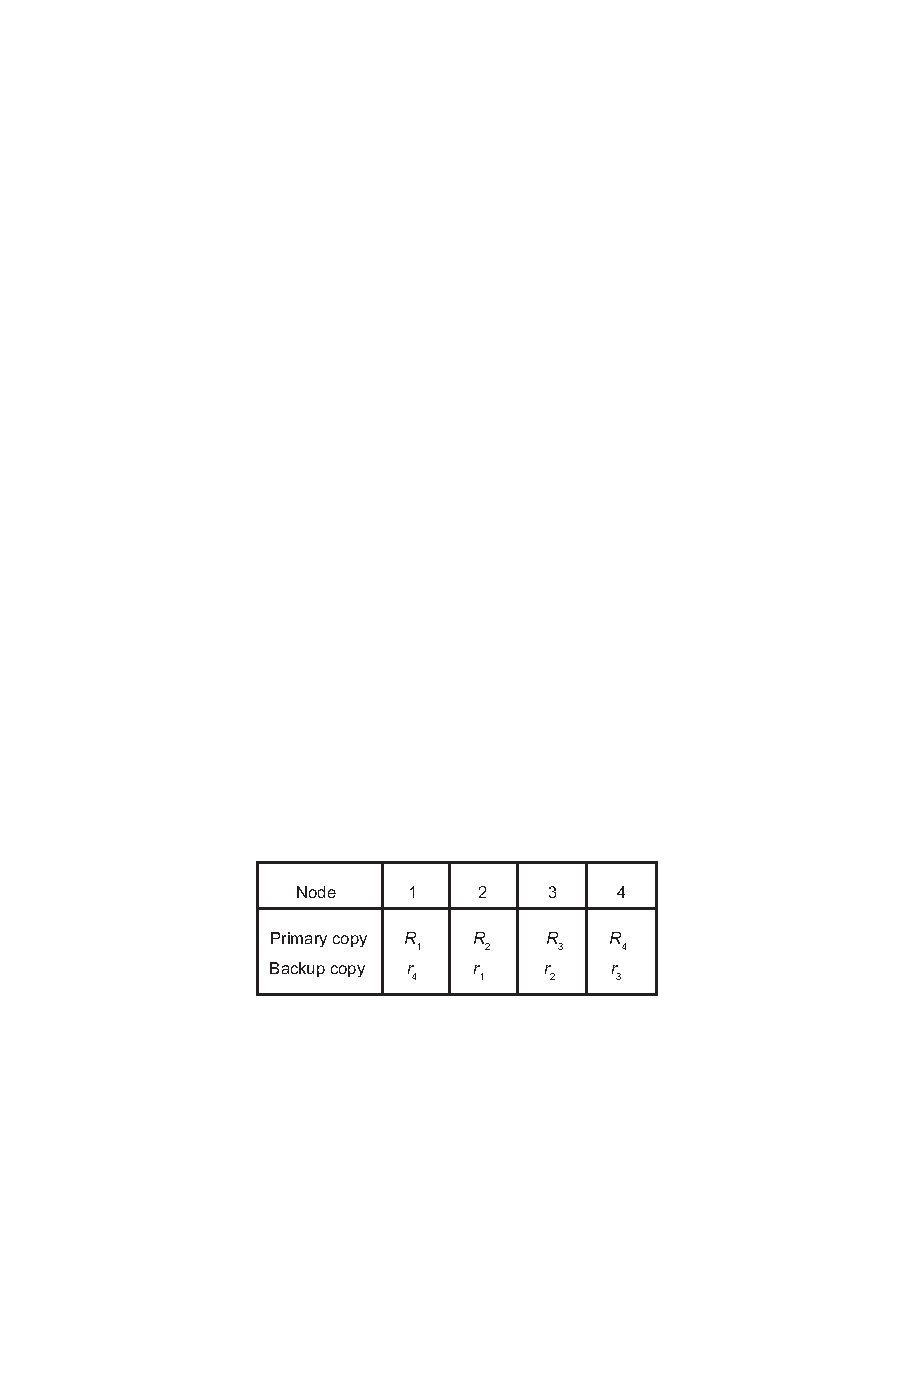
\includegraphics[width=0.48\textwidth]{chained}
\caption{Example of Chained Partitioning.}
\label{fig:chained}
\end{figure}

\section{Conclusion}
Parallel database systems strive to exploit multiprocessor architectures using software-oriented solutions for data management. Their promises are high-performance, high-availability, and extensibility with a good cost/performance ratio. Furthermore, parallelism is the only viable solution for supporting very large databases within a single system.

Parallel data management techniques extend distributed database techniques in order to obtain high-performance, high-availability, and extensibility. Essentially, the solutions for transaction management, i.e., distributed concurrency control, reliability, atomicity, and replication can be reused. However, the critical issues for such architectures are data placement, parallel query execution, parallel data processing, parallel query optimization and load balancing. 

The solutions to these issues are more involved than in distributed DBMS because the number of nodes may be much higher. Furthermore, parallel data management techniques use different assumptions such as fast interconnect and homogeneous nodes that provide more opportunities for optimization.

\bibliographystyle{abbrv}
\bibliography{sqlonhadoop}

\end{document}
